%%%%%%%%%%%%%%%%%%%%%%%%%%%%%%%%%%%%%%%%%
% Thin Sectioned Essay
% LaTeX Template
% Version 1.0 (3/8/13)
%
% This template has been downloaded from:
% http://www.LaTeXTemplates.com
%
% Original Author:
% Nicolas Diaz (nsdiaz@uc.cl) with extensive modifications by:
% Vel (vel@latextemplates.com)
%
% License:
% CC BY-NC-SA 3.0 (http://creativecommons.org/licenses/by-nc-sa/3.0/)
%
%%%%%%%%%%%%%%%%%%%%%%%%%%%%%%%%%%%%%%%%%

%----------------------------------------------------------------------------------------
%	PACKAGES AND OTHER DOCUMENT CONFIGURATIONS
%----------------------------------------------------------------------------------------

\documentclass[a4paper, 11pt]{article} % Font size (can be 10pt, 11pt or 12pt) and paper size (remove a4paper for US letter paper)

\usepackage[protrusion=true,expansion=true]{microtype} % Better typography
\usepackage{graphicx} % Required for including pictures
\usepackage{wrapfig} % Allows in-line images
\renewcommand{\figurename}{Figura} % Modifica del Caption default delle figure
\usepackage{mathpazo} % Use the Palatino font
\usepackage[T1]{fontenc} % Required for accented characters
\usepackage{afterpage}
\usepackage{hyperref}
\usepackage{pdfpages}
\usepackage{graphicx}
\usepackage{float}
\usepackage{xcolor}
\usepackage{listings}
\renewcommand{\contentsname}{Indice}
\renewcommand{\refname}{Bibliografia}

\newcommand\blankpage{%
    \null
    \thispagestyle{empty}%
    \addtocounter{page}{-1}%
    \newpage}
    
\linespread{1.05} % Change line spacing here, Palatino benefits from a slight increase by default

\makeatletter
\renewcommand\@biblabel[1]{\textbf{#1.}} % Change the square brackets for each bibliography item from '[1]' to '1.'
\renewcommand{\@listI}{\itemsep=0pt} % Reduce the space between items in the itemize and enumerate environments and the bibliography

\renewcommand{\maketitle}{ % Customize the title - do not edit title and author name here, see the TITLE block below
\begin{flushright} % Right align
{\LARGE\@title} % Increase the font size of the title

\vspace{100pt} % Some vertical space between the title and author name

{\large\@author} % Author name
\\\@date % Date

\vspace{100pt} % Some vertical space between the author block and abstract
\end{flushright}
}

%----------------------------------------------------------------------------------------
%	TITLE
%----------------------------------------------------------------------------------------

\title{\textbf{Progetto Programmazione Java}\\ % Title
Servizio di Messaggistica Istantanea} % Subtitle

\author{Rambod Rahmani % Author
\\{\textit{rambodrahmani@autistici.org}}  % Institution
\\{\textit{Relentlessly pursue knowledge and selflessly share it with others.}}\vspace{3mm}}

\date{\today} % Date

%----------------------------------------------------------------------------------------

\begin{document}

%----------------------------------------------------------------------------------------
%	OPEN ACCESS MANIFESTO
%----------------------------------------------------------------------------------------

Il materiale che troverai in questo documento \`e completamente gratuito. Per quanto riguarda il contenuto, dato che non \`e stato rivisto da "esperti", mi preme precisare che NON garantisco in alcun modo la correttezza totale.\\
\\
Il documento \`e rilasciato sotto i termini della licenza Creative Commons Attribuzione - Non commerciale - Condividi allo stesso modo 3.0 Italia. Per visionare una copia completa della licenza, visita \\
http://creativecommons.org/licenses/by-nc-sa/3.0/it/legalcode.\\
\\
Lo scopo di tutto ci\`o non \`e tanto arricchire il mio curriculum personale, bens\`i condividere le mie conoscenze con il maggiore numero di persone possibile. Considera questo documento anche come un invito a pubblicare e condividere i tuoi saperi, perch\'e il fondamento di una vera formazione \`e il libero accesso al sapere in tutte le sue forme.\\
\\
\begin{center}
\textit{"Information is power. But like all power, there are those who want to keep it for themselves.\\
...\\
Those with access to these resources - students, librarians, scientists - you have been given a privilege.\\
...\\
Meanwhile, those who have been locked out are not standing idly by. You have been sneaking through holes and climbing over fences, liberating the information locked up by the publishers and sharing them with your friends. But all of this action goes on in the dark, hidden underground. \textbf{It's called stealing or piracy, as if sharing a wealth of knowledge were the moral equivalent of plundering a ship and murdering its crew.} But sharing isn't immoral - it's a moral imperative. Only those blinded by greed would refuse to let a friend make a copy.\\
...\\
There is no justice in following unjust laws. It's time to come into the light and, in the grand tradition of civil disobedience, declare our opposition to this private theft of public culture.\\
...\\
With enough of us, around the world, we'll not just send a strong message opposing the privatization of knowledge - we'll make it a thing of the past. Will you join us?"\\}
\end{center}
\begin{flushright}
Guerilla Open Access Manifesto\\
Aaron Swartz
\end{flushright}

\afterpage{\blankpage}

\newpage
\maketitle % Print the title section

%----------------------------------------------------------------------------------------
%	ABSTRACT AND KEYWORDS
%----------------------------------------------------------------------------------------

%\renewcommand{\abstractname}{Summary} % Uncomment to change the name of the abstract to something else

\begin{abstract}
Il presente documento contiene la documentazione prodotta durante la realizzazione del Progetto "Servizio di Messaggistica Istantanea" per l'esame di "Programmazione Java" - Prof. Mario G.C.A. Cimino - presso l'universit\`a degli studi di Pisa - Ingegneria Informatica.\\
Il progetto Java \`e disponibile open source su GitHub: \textcolor{blue}{\url{https://github.com/rambodrahmani/esame-programmazione-java}}
\end{abstract}

\hspace*{3,6mm}\textit{Keywords:} programmazione , java , esame , unipi , rambod , rahmani % Keywords

\vspace{30pt} % Some vertical space between the abstract and first section

\afterpage{\blankpage}

\newpage

\vspace*{\fill}
	\begin{center}
		\begin{em}
			Dedicato a mia madre Sara, mio padre Magid e mio fratello gemello Ramtin per esserci stati quando ho avuto bisogno e per avermi reso la persona che sono oggi.
		\end{em}
	\end{center}
\vspace*{\fill}

\afterpage{\blankpage}

\newpage

\tableofcontents

%----------------------------------------------------------------------------------------
%	ESSAY BODY
%----------------------------------------------------------------------------------------

\newpage
\section{Introduzione}

Il progetto che ho sviluppato per l'esame di Programmazione Java \`e un software di messaggistica istantanea che permetto di scambio di messaggi di testo tra due Client connessi contemporaneamente. Il progetto comprende anche un Server di Log che riceve messaggi di Log, relativi all'utilizzo della GUI, da parte dei vari Client connessi al servizio di messaggistica.\\
\\
Il documento si sviluppa secondo le varie fasi di sviluppo del Progetto.\\
Le fasi di lavoro sono state preimpostate dalle consegne d'esame pubblicate dal professore.\\
\\
Il codice sorgente del prodotto e gli altri File prodotti durante lo sviluppo sono disponibili al seguente indirizzo: GitHub - \textcolor{blue}{\url{https://github.com/rambodrahmani/esame-programmazione-java}}

%------------------------------------------------

\newpage
\section{Analisi}

Il progetto consiste nella realizzazione di un applicativo che permetta lo scambio di messaggi di testo.\\
\\
Il progetto \`e composto da:
\begin{itemize}
\item \textbf{Server di Log}: che si occupa di ricevere i logs, relativi alla navigazione nell'interfaccia utente, dai Clients. Il Server di Log valida il singolo log XML ricevuto dal Client e lo salva in un file di testo (file di log aperto);
\item \textbf{Client}: Il client \`e la parte del progetto che permette lo scambio di messaggi di testo. Dotato di interfaccia grafica, permette di visualizzare i Contatti connessi, aprire nuove finestre di conversazione e accedere al diagramma a torta UML.
\end{itemize}

\subsection{Server di Log}

Il Server di Log non ha interfaccia grafica. Si occupa di ricevere e conservare, su file di testo locale, i vari logs XML dai Clients connessi.\\
\\
\textbf{Vista Dinamica}
\begin{enumerate}
\item All'avvio, il Server di Log carica da file di configurazione locale i parametri presenti. 
\item Una volta avviato il Server, l'applicativo rimane in attesa di connessioni da parte dei vari Clients;
\item Valida i singoli logs XML quando ricevuti dai Clients;
\item Appende su file di testo locale (file di log aperto) i singoli XML validati;
\item Alla chiusura, disconnette i vari Clients connessi e termina.
\end{enumerate}
\vspace{0.5cm}
\textbf{File di Configurazione Locale in XML}\\
All'avvio del sistema, il Server carica dal file di configurazione locale:
\begin{enumerate}
\item La porta da utilizzare per avviare il Server;
\item La locazione del file di Log locale;
\item La locazione del file XSD da utilizzare per validare i singoli log.
\end{enumerate}
\vspace{0.5cm}
\textbf{Messaggio di Log}\\
Ogni messaggio di Log contiene:
\begin{enumerate}
\item L'indirizzo email del Contatto che lo ha inviato;
\item Il tipo di evento;
\item Data e ora dell'invio da parte del Contatto.
\end{enumerate}
\vspace{0.5cm}
\textbf{File di Log di Testo}\\
Il Sistema riceve e registra un log per i seguenti eventi:
\begin{enumerate}
\item Eventi relativi all'utilizzo dell'interfaccia grafica, inviati da parte dei Client.
\end{enumerate}

\subsection{Client}

Il Client ha interfaccia grafica. Permette all'utente di visualizzare i Contatti connessi, aprire nuove conversazioni con questi, inviare e ricevere messaggi ed accedere al diagramma a Torta nella finestra Statistiche.\\
\\
\textbf{Vista Dinamica}
\begin{enumerate}
\item All'avvio dell'applicativo, il Client legge dal file di configurazione locale i parametri presenti;
\item Quando l'utente preme il pulsante "Connetti", il Client si connette al Server di Log e si registra nella Base di Dati con l'email inserita;
\item Il Client legge da Base di Dati i Contatti connessi e li carica nella Tabella "Contatti";
\item Il Client attende le connessioni da parte dei vari Contatti;
\item A intervalli di tempo determinati, il Client aggiorna la lista Contatti connessi;
\item Lo stato di connessione viene aggiornato impostando il testo della Stringa "Stato" che si trova sotto la lista dei Contatti;
\item L'utente pu\`o aprire una nuova finestra di conversazione con un Contatto facendo doppio Click sul nome del contatto nella lista Contatti;
\item La finestra di conversazione aperta permette lo scambio di messaggi con il Contatto selezionato;
\item L'utente pu\`o utilizzare il menu "Strumenti" per accedere alla finestra "Statistiche";
\item La finestra statistiche contiene un diagramma a torta che rappresenta le ore di attivit\`a dei 5 Contatti pi\`u connessi;
\item Alla chiusura del Client, il Contatto viene rimosso dalla Base di Dati, si disconnette dal Server di Log e termina;
\item Alla disconnessione di un Client dal servizio di messaggistica:
\begin{enumerate}
\item Vengono notificati della sua disconnessione, oltre che il Server di Log, tutti i Client che hanno una conversazione aperta con esso.
\item Vengono aggiornate le ore di attivit\`a nella tabella "storico" della Base di dati.
\end{enumerate}
\end{enumerate}
\vspace{0.5cm}
\textbf{File di Configurazione Locale in XML}\\
All'avvio del sistema, il Client carica dal file di configurazione locale:
\begin{enumerate}
\item Indirizzo e porta del Server di Log a cui connettersi;
\item La porta su cui avviare il Client;
\item L'indirizzo, la porta, il nome utente e la password da utilizzare per accedere alla Base di dati;
\item Il numero di ultimi messaggi di ciascuna conversazioni da salvare in Cache.
\end{enumerate}
\vspace{0.5cm}
\textbf{Cache Locale}\\
Alla chiusura di una finestra di conversazione con un Contatto, il Sistema salva su file binario gli ultimi N messaggi scambiati. All'avvio della successiva conversazione con il Contatto, carica dal suddetto file gli ultimi N messaggi.\\
\\
\textbf{Base di Dati}\\
Il Sistema archivia le seguenti informazioni su base di dati:
\begin{enumerate}
\item Connessione e disconnessione dei vari Client (email, indirizzo IP, data e ora);
\item I messaggi inviati dai vari Client (mittente, destinatario, messggio, data e ora).
\item Il numero di ore che ogni Contatto spende connesso al Servizio di Messaggistica.
\end{enumerate}
\vspace{0.5cm}
\textbf{Struttura Tabelle Base di Dati}\\
\\
\underline{Contatti}
\lstset{language=sql}
\begin{lstlisting}[frame=single]
contatti (email, indirizzo_ip, data)
email: VARCHAR(45), PRIMARY KEY,
indirizzo_ip: VARCHAR(45),
data: TIMESTAMP
\end{lstlisting}
La tabella Contatti contiene gli indirizzi Email dei vari Clients connessi e l'indirizzo IP a questi associato.\\
Ogni contatto \`e caratterizzato da un indirizzo Email, da un indirizzo IP e dall'ora in cui si \`e connesso.\\
Non \`e possibile che due o pi\`u contatti con lo stesso indirizzo Email possano connettersi.\\
\\
\underline{Messaggi}
\lstset{language=sql}
\begin{lstlisting}[frame=single]
messaggi (id, mittente, destinatario, testo, data)
id: INT(45), PRIMARY KEY,
mittente: VARCHAR(45),
destinatario: VARCHAR(45),
testo: MEDIUMTEXT,
data: TIMESTAMP
\end{lstlisting}
La tabella Messaggi contiene i messaggi scambiati tra i vari Contatti.\\
Ogni messaggio \`e composto da un id numerico (ho preferito utilizzare una colonna chiave dedicata perch\`e altrimenti si dovrebbe coinvolgere tutte le colonne della tabella per ottenere una chiave univoca), l'indirizzo email del mittente, l'indirizzo email del destinatario, il testo del messaggio e la data e l'ora in cui \`e stato spedito.\\
\\
\underline{Storico}
\lstset{language=sql}
\begin{lstlisting}[frame=single]
storico (email, durata)
email: VARCHAR(45), PRIMARY KEY,
durata: DOUBLE
\end{lstlisting}
La tabella Storico contiene, per ciascun Client, l'email e il numero di ore spese connesso.
Viene utilizzata dai vari Clients per generare il diagramma a Torta.\\
Ogni volta che un Client si disconnette, viene utilizzata la colonna data della tabella contatti per calcolare il numero di ore che il Client \`e rimasto connesso.\\
\\
\textbf{File di Log remoto}\\
Il Sistema invia un log per i seguenti eventi:
\begin{enumerate}
\item Quando l'utente preme il pulsante "Connetti" per avviare il Client;
\item Quando l'utente preme il pulsante "Disconnetti" per fermare il Client;
\item Quando l'utente accede al menu "Strumenti";
\item Quando l'utente accede al sotto-menu "Statistiche" (Strumenti $\rightarrow$ Statistiche) aprendo il frame Statistiche;
\item Quando l'utente apre una nuova finestra di conversazione con doppio click sulla tabella "Contatti";
\item Quando un Client invia un messaggio premendo sul pulsante "Invia" del Frame conversazione.
\end{enumerate}
\vspace{0.5cm}
\textbf{Interfaccia grafica disegnata per il Client:}
\afterpage{
\clearpage
\begin{figure}
\vspace{-4.4cm}
\hspace{-4.0cm}
\includegraphics[width=1.56\textwidth]{images/analisi_client.png}
\caption{Interfaccia Grafica Client}
\end{figure}
\thispagestyle{empty}
\clearpage
}

%------------------------------------------------

\newpage
\section{Progetto}

\subsection{Server di Log}

Le classi del Server di Log, come mostrate graficamente nel diagramma UML, sono le seguenti:\\
\\
\textbf{Classe Server}\\
Classe contenente la funzione main() del progetto.\\
Gestisce l'Input/Output da terminale per la gestione (avvio, stampa logs, stampa lista Client connessi, arresto) del Server di Log.\\
\\
\textbf{Classe ParametriConfigurazione}\\
Contiene i parametri di configurazione letti dal file di configurazione .xml locale.\\
Utilizzato dalla classe GestoreParametriConfigurazioneXML.\\
Serializzata/Deserializzata tramite XMLStream.\\
\\
\textbf{Classe GestoreParametriConfigurazioneXML}\\
Legge i parametri di configurazione dal file di configurazione .xml locale.\\
Valida i parametri tramite XML Schema con file .xsd locale.\\
Salva i parametri di configurazione in una istanza statica della classe ParametriConfigurazione.\\
\\
\textbf{Classe GestoreLogsXML}\\
Gestisce l'accesso sincronizzato di lettura e scrittura sul file di log .txt locale.\\
Valida i log ricevuti tramite XML Schema con file .xsd locale.\\
\\
\textbf{Classe ThreadServerSocket}\\
Estende Thread.\\
Gestisce il ServerSocket in attesa delle connessioni da parte dei Client.\\
\\
\textbf{Classe SocketClient}\\
Estende Thread.\\
Gestisce il Socket di comunicazione tra Server di Log e ciascun Client connesso.\\
\\
\textbf{Diagramma UML:}\\
\textbf{N.B: I file PDF dei diagrammi UML sono disponibili singolarmente nella cartella "2 - Progetto".}
\clearpage
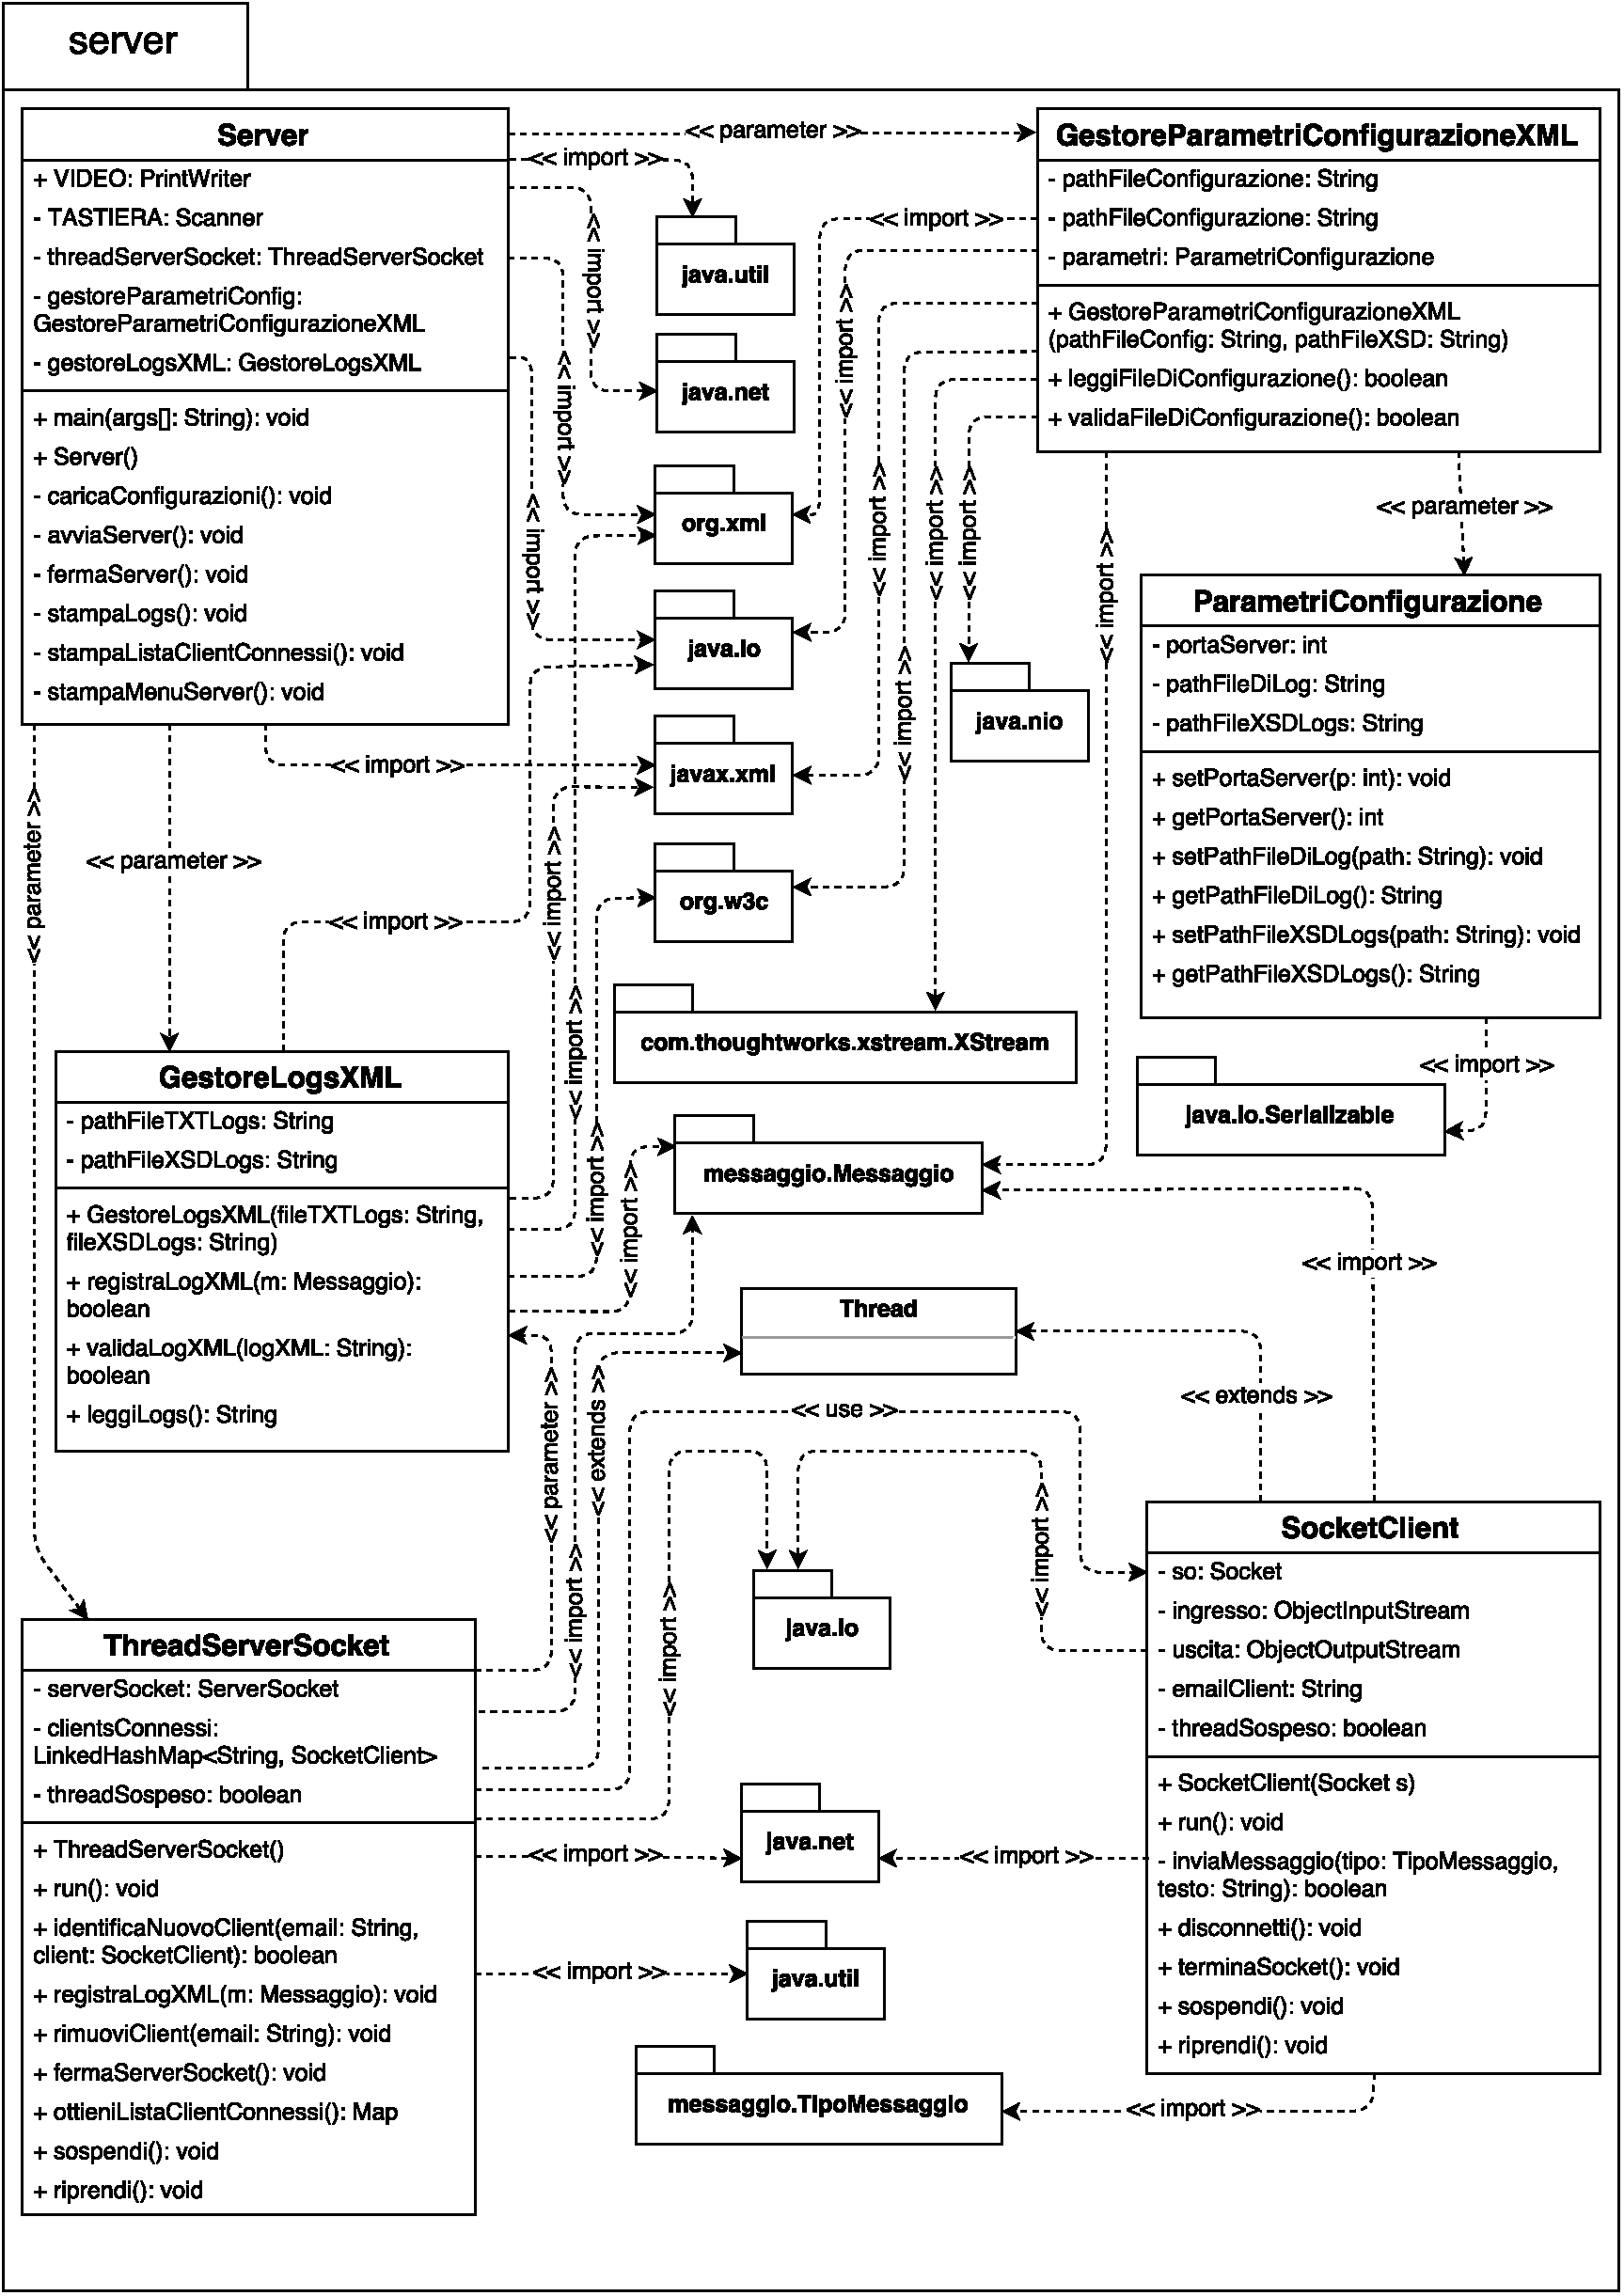
\includepdf[scale=0.98,offset=1 0,pagecommand=\thispagestyle{empty}]{diagrammi/server.pdf}

\subsection{Client}

Le classi del Client, come mostrate graficamente nel diagramma UML, sono le seguenti:\\
\\
\textbf{Classe Client}\\
Classe contenente la funzione main() del progetto.\\
Carica i parametri di configurazione utilizzando la classe GestoreParametriDiConfigurazione.\\
Se la lettura dei parametri di configurazione termina con success, istanzia una variabile di tipo FrameContatti contenente la GUI principale del progetto.\\
\\
\textbf{Classe Contatto}\\
Contiene le informazioni di ciascun Contatto connesso.\\
Utilizzata dalla classe GestoreBaseDiDati per ottenere la lista dei contatti connessi.\\
\\
\textbf{Classe FrameContatti}\\
Contiene il JFrame con la GUI principale (area connessione, lista contatti connessi, menu strumenti).\\
Istanzia una variabile di tipo ServerSocketConversazioni che avvia un ServerSocket che rimane in ascolto delle connessione da parte degli altri Contatti.\\
\\
\textbf{Classe FrameConversazione}\\
Contiene il JFrame con la GUI della finestra di conversazione.\\
Istanzia una variabile di tipo SocketConversazione che si connette al  ServerSocketConversazioni del contatto con cui si desidera conversare.\\
\\
\textbf{Classe FrameStatistiche}\\
Contiene il JFrame con la GUI della finestra delle statistiche.\\
Carica il pannello JavaFX contenente il diagramma a Torta delle statistiche.\\
\\
\textbf{Classe GestoreBaseDiDati}\\
Esegue tutte le query sulla Base di Dati.\\
\\
\textbf{Classe GestoreCacheConversazioni}\\
Si occupa di salvare e prelevare da file binario locale gli ultimi messaggi scambiati con ciascun Contatto.\\
\\
\textbf{Classe GestoreParametriConfigurazioneXML}\\
Legge i parametri di configurazione dal file di configurazione .xml locale.\\
Valida i parametri tramite XML Schema con file .xsd locale.\\
\\
\textbf{Classe ParametriConfigurazione}\\
Contiene i parametri di configurazione letti dal file di configurazione .xml locale dalla classe GestoreParametriConfigurazioneXML.\\
Serializzata/Deserializzata tramite XMLStream.\\
\\
\textbf{Classe ModelloTabellaContatti}\\
Estende AbstractTableModel.\\
Implementa i metodi per AbstractTableModel.\\
Gestisce i dati della tabella contenente la lista dei Contatti connessi.\\
\\
\textbf{Classe ServerSocketConversazioni}\\
Gestisce il ServerSocket in attesa delle connessioni da parte degli altri Contatti.\\
Estende Thread.\\
\\
\textbf{Classe SocketConversazione}\\
Gestisce il Socket di comunicazione tra due Clients connessi che scambiano messaggi.\\
Estende Thread.\\
\\
\textbf{Classe SocketServerDiLog}\\
Gestisce il Socket di comunicazione con il Server di Log.\\
Estende Thread.\\
\\
\textbf{Classe Storico}\\
Contiene le informazioni riguardanti il numero di ore di connessione per ciascun Contatto.\\
Utilizzata dalla classe GestoreBaseDiDati per ottenere la lista delle ore spese connesse per ciascun contatti.\\
\\
\textbf{Diagramma UML:}\\
\textbf{N.B: I file PDF dei diagrammi UML sono disponibili singolarmente nella cartella "2 - Progetto".}
\clearpage
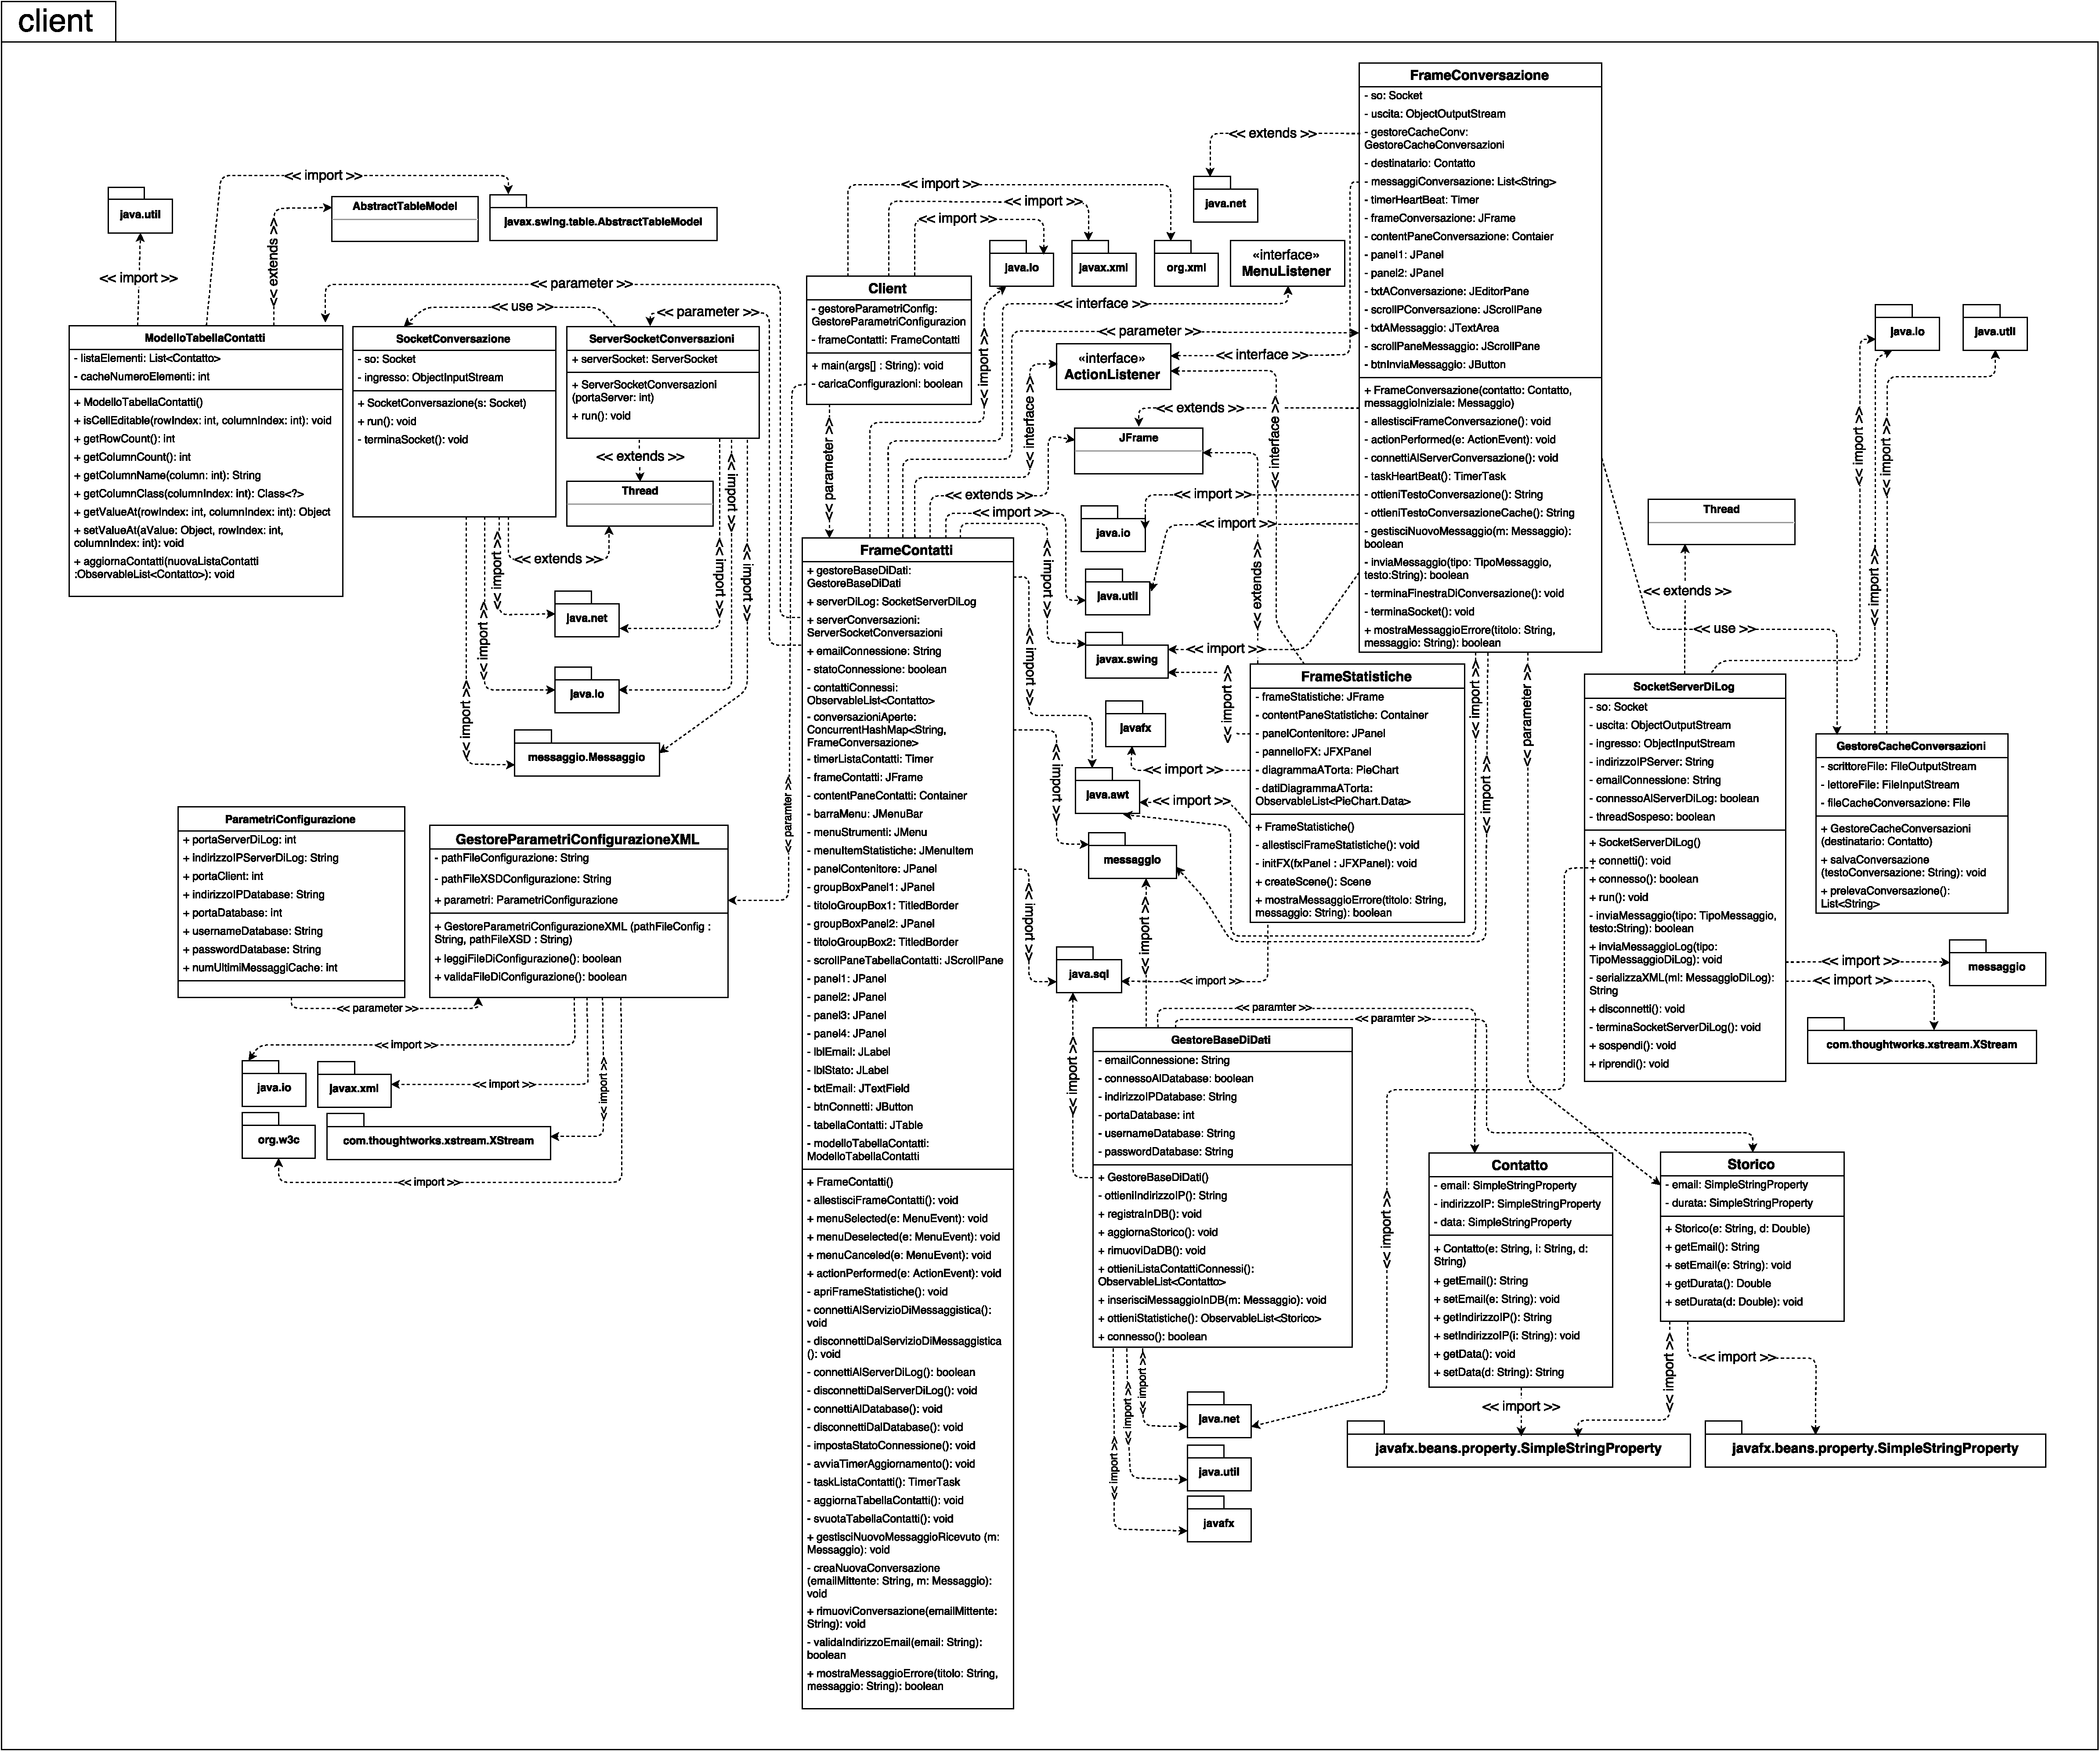
\includepdf[scale=0.98,offset=1 0,pagecommand=\thispagestyle{empty}]{diagrammi/client.pdf}

\subsection{Classi Comuni}

Client e Server di Log hanno in comune il package messaggio, che contiene le classi Messaggio, MessaggioDiLog, TipoMessaggio e TipoMessaggioDiLog, e che verr\`a sviluppato sotto forma di una Java Class Library, in modo da ottenere un .jar da includere nei due progetti che ne necessitano.\\
Essendo messaggio l'oggetto serializzato che viene scritto e letto da ObjectOutputStream e ObjectInputStream, conviene avere un unico file .jar da includere nel progetto Server e Client in modo da non incorrere in errori di incongruenza.\\
\\
\textbf{Classe Messaggio}\\
Implementa Serializable.\\
Contiene i campi di ciascun messaggio scambiato tra Server e Client o tra due Client.\\
\\
\textbf{Classe TipoMessaggio}\\
Implementa Serializable.\\
Enumerazione contenente i tipi di messaggio che possono essere creati.\\
\\
\textbf{Classe MessaggioDiLog}\\
Implementa Serializable.\\
Contiene i campi di ciascun messaggio di log inviato dai Client al Server di Log.\\
\\
\textbf{Classe TipoMessaggioDiLog}\\
Implementa Serializable.\\
Enumerazione contenente i tipi di messaggio di log che possono essere creati.\\
\\
\textbf{Diagramma UML:}\\
\textbf{N.B: I file PDF dei diagrammi UML sono disponibili singolarmente nella cartella "2 - Progetto".}
\clearpage
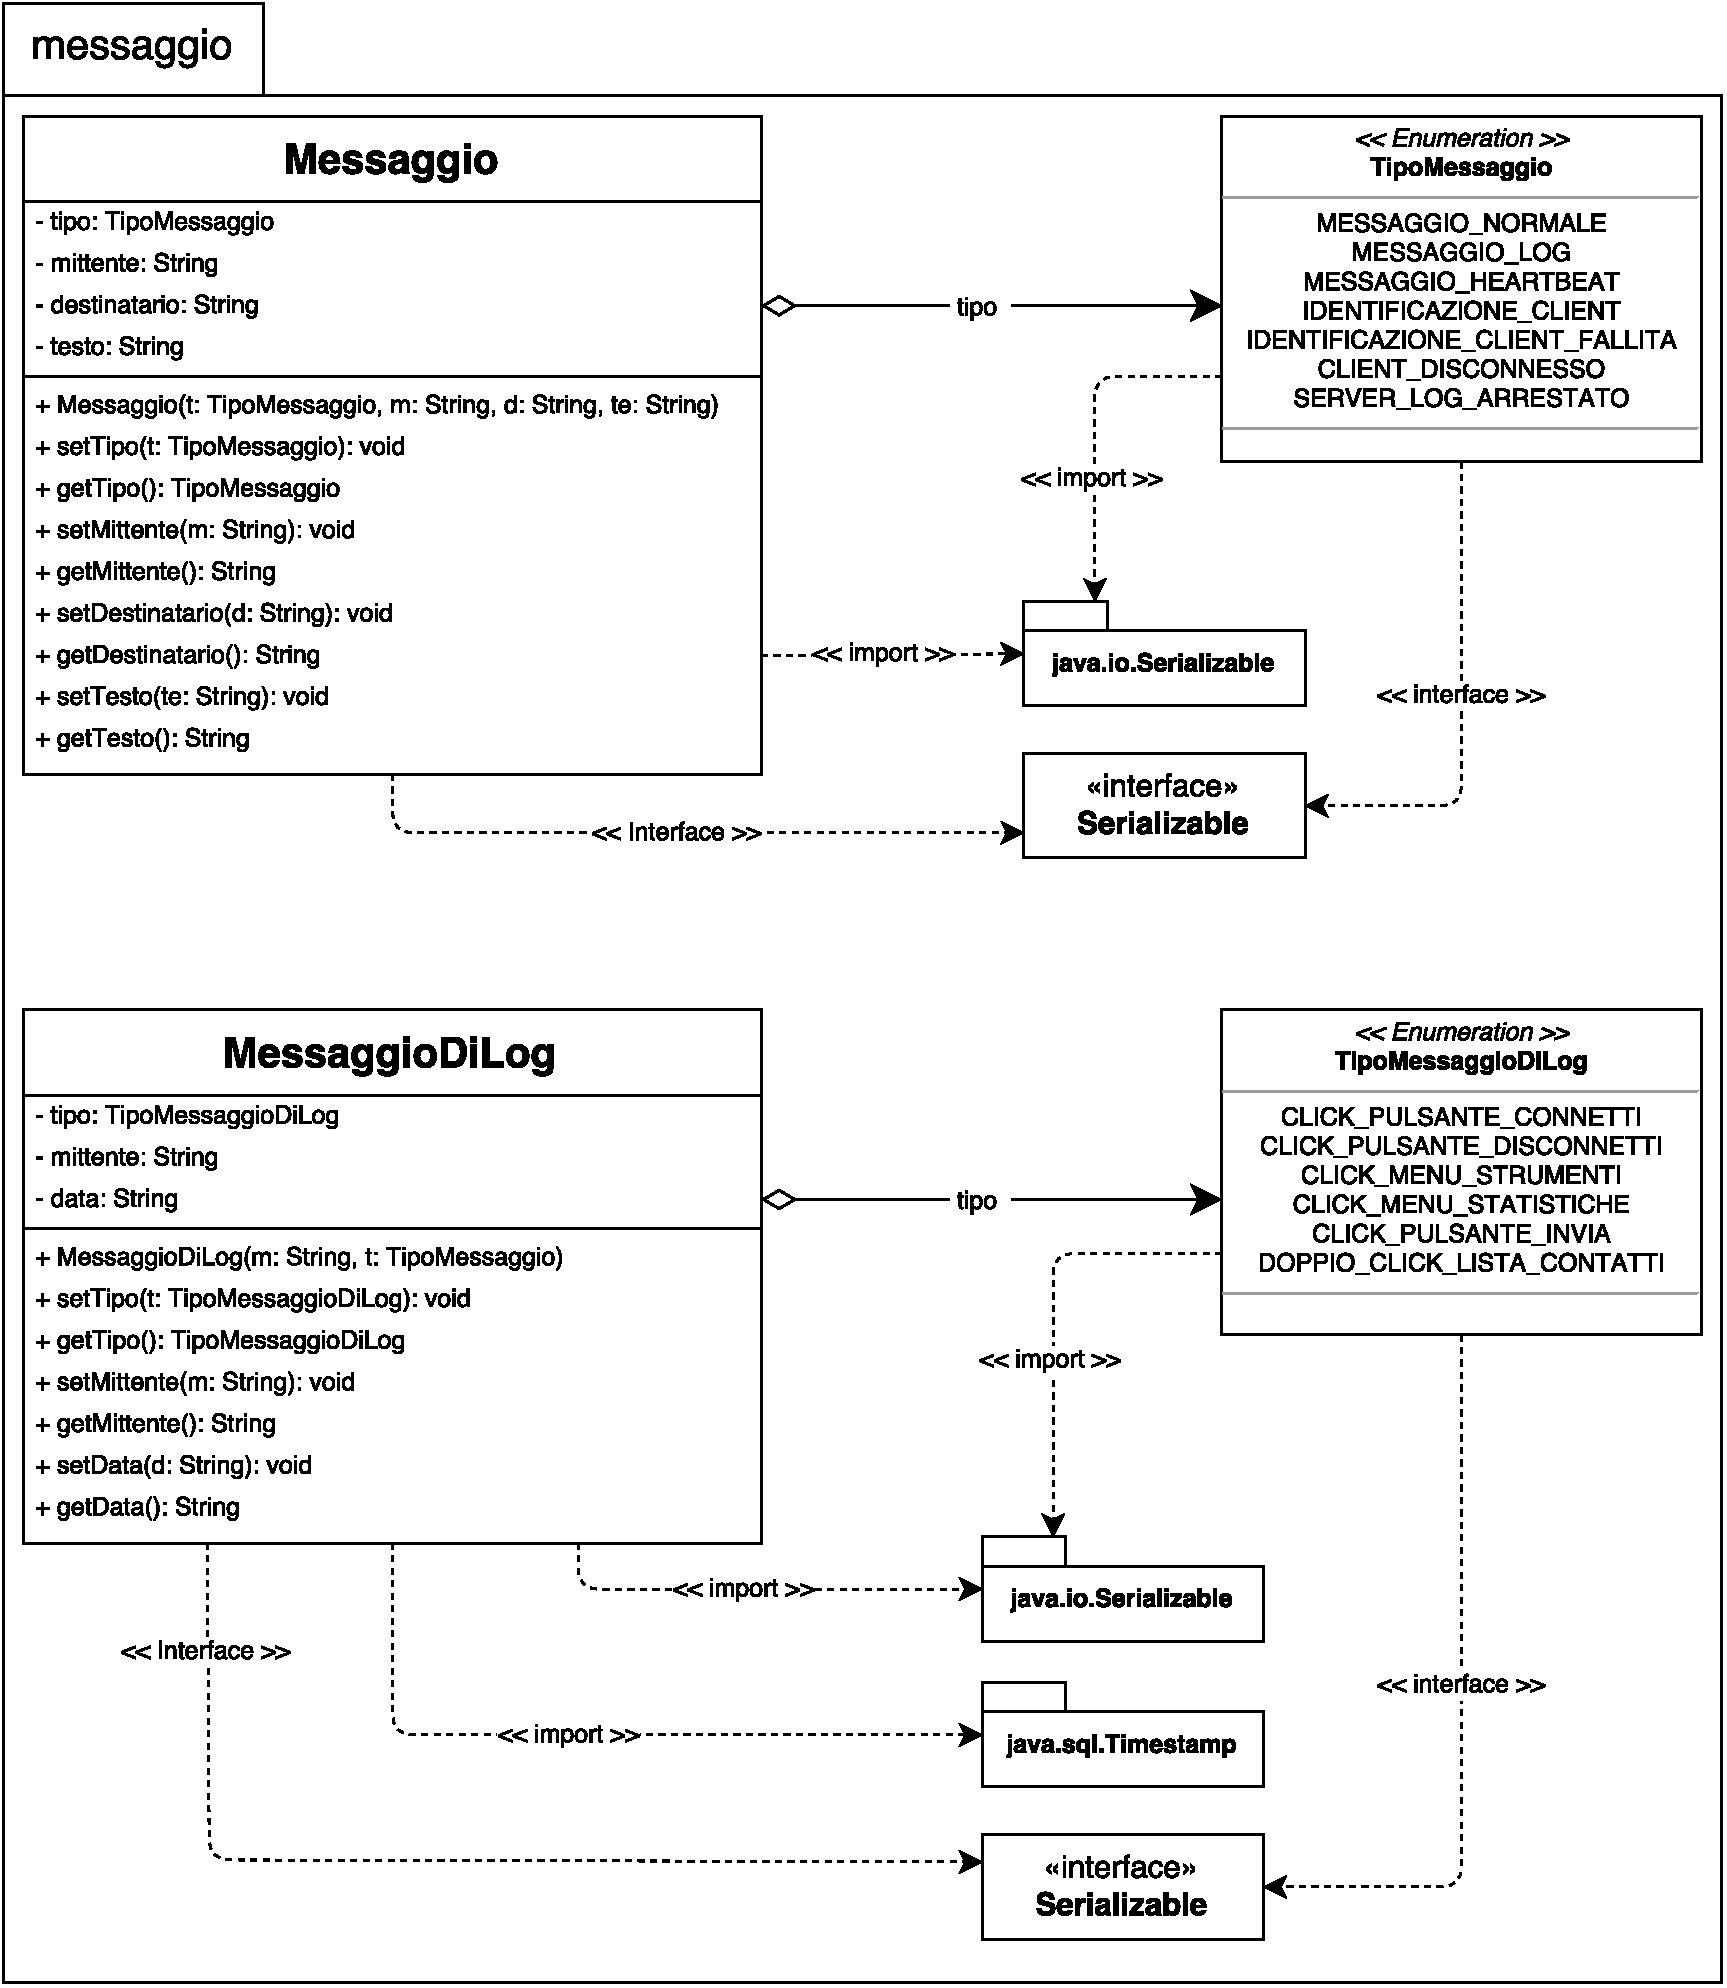
\includepdf[scale=0.98,offset=1 50,pagecommand=\thispagestyle{plain}]{diagrammi/serverclient.pdf}
%------------------------------------------------

\newpage
\section{Manuale d'uso}

Il presente manuale d'uso spiega come utilizzare il Server di Log e il Client del progetto.\\
\\
Il Server di Log non ha interfaccia grafica e pu\`o essere gestito utilizzando la linea di comando, mentre il Client ha un'interfaccia grafica composta da differenti finestre di controllo.

\subsection{Server di Log}

Prima di avviare il Server di Log assicurarsi che:
\begin{enumerate}
\item Il file configurazione.xml sia presente nella cartella da cui viene eseguito il Server di Log.
\item Il file configurazione.xsd sia presente nella cartella da cui viene eseguito il Server di Log.
\item Il file validaLogs.xsd sia presente nella cartella da cui viene eseguito il Server di Log.
\item Siano stati inseriti i parametri corretti nel file configurazioni.xml.
\end{enumerate}
\vspace{0.5cm}
Il Server di Log pu\`o essere avviato da linea di comando con il seguente comando:
\lstset{language=bash}
\begin{lstlisting}[frame=single]
$ java -jar Server.jar
\end{lstlisting}
\textbf{Oppure \`e possibile utilizzare lo script .bat, vedi sezione 4.3.}\\
\clearpage
\hspace{-0.8cm}
Una volta avviato il Server di Log da linea di comando, verr\`a stampato il seguente Menu su terminale:\\
\begin{center}
\begin{figure}[H]
\vspace{-1.0cm}
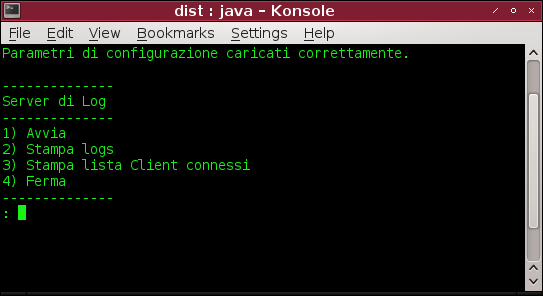
\includegraphics[width=1.0\textwidth]{images/server_di_log-1.png}
\vspace{-0.6cm}
\caption{Avvio Server di Log}
\end{figure}
\end{center}
Il Server di Log pu\`o essere avviato con input 1:\\
\vspace{-0.6cm}
\begin{center}
\begin{figure}[H]
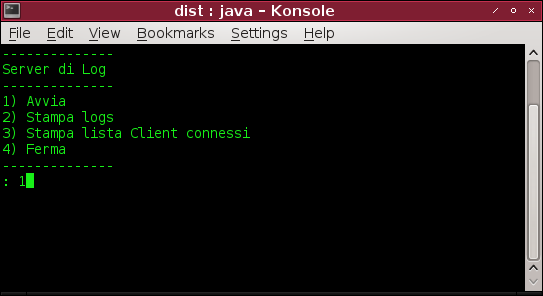
\includegraphics[width=1.0\textwidth]{images/server_di_log-2.png}
\vspace{-0.6cm}
\caption{Avvio Server di Log}
\end{figure}
\end{center}
\begin{center}
\begin{figure}[H]
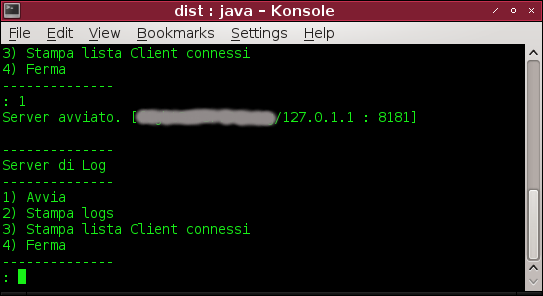
\includegraphics[width=1.0\textwidth]{images/server_di_log-3.png}
\vspace{-0.6cm}
\caption{Avvio Server di Log}
\end{figure}
\end{center}
\vspace{-0.6cm}
In questo stato il Server di Log rimane in attesa di comandi e stampa messaggi relativi agli eventi che si verificano:
\vspace{-0.6cm}
\begin{center}
\begin{figure}[H]
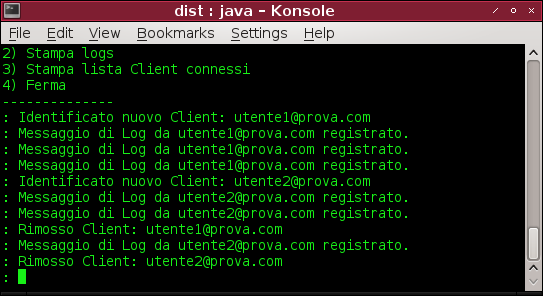
\includegraphics[width=1.0\textwidth]{images/server_di_log-4.png}
\vspace{-0.6cm}
\caption{Eventi Server di Log}
\end{figure}
\end{center}
Con l'input 2 possiamo stampare tutti i messaggi di Log ricevuti dai vari Client dal momento dell'avvio del Server di Log:\\
\vspace{-0.8cm}
\begin{center}
\begin{figure}[H]
\vspace{-2.0cm}
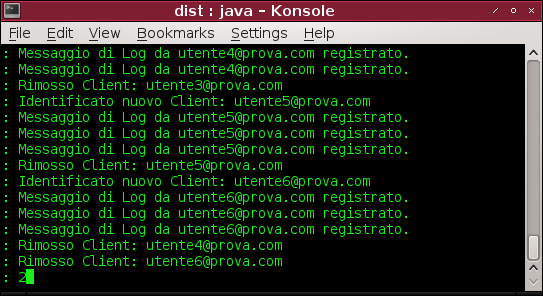
\includegraphics[width=1.0\textwidth]{images/server_di_log-5.png}
\\
\\
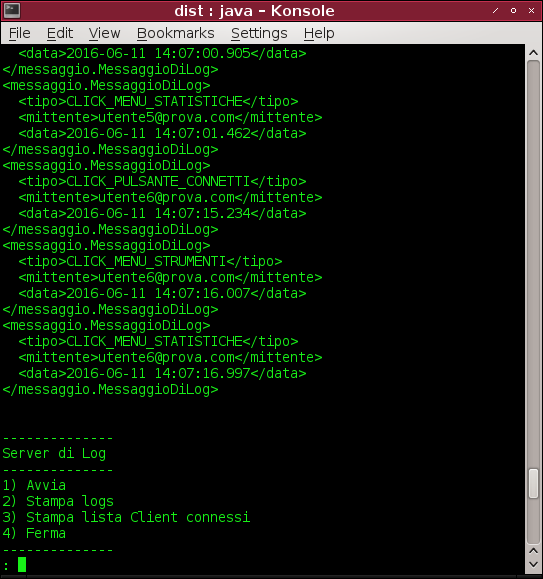
\includegraphics[width=1.0\textwidth]{images/server_di_log-6.png}
\vspace{-0.6cm}
\caption{Stampa Logs Server di Log}
\end{figure}
\end{center}
\vspace{-1.0cm}
Con l'input 3 \`e possibile stampare la lista dei Client connessi al Server di Log al momento:\\
\vspace{-0.8cm}
\begin{center}
\begin{figure}[H]
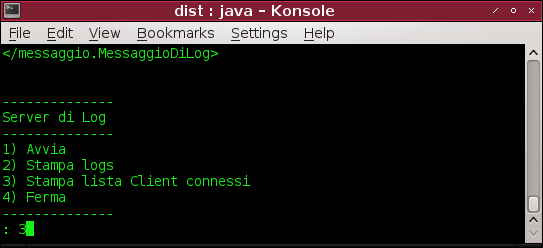
\includegraphics[width=1.0\textwidth]{images/server_di_log-7.png}
\vspace{-0.6cm}
\caption{Stampa Client connessi Server di Log}
\end{figure}
\end{center}
\begin{center}
\begin{figure}[H]
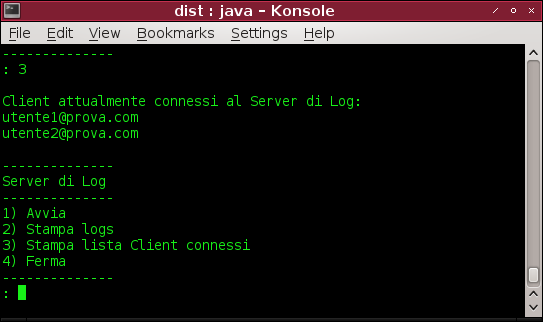
\includegraphics[width=1.0\textwidth]{images/server_di_log-8.png}
\vspace{-0.6cm}
\caption{Stampa Client connessi Server di Log}
\end{figure}
\end{center}
Con l'input 4 possiamo arrestare il Server di Log (viene richiesta conferma prima di procedere):\\
\vspace{-0.6cm}
\begin{center}
\begin{figure}[H]
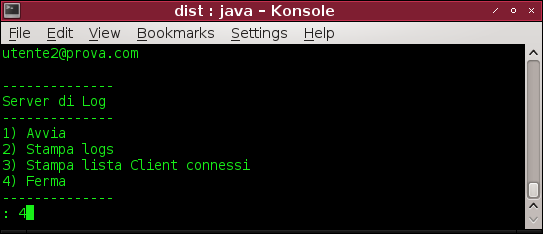
\includegraphics[width=1.0\textwidth]{images/server_di_log-9.png}
\vspace{-0.6cm}
\caption{Arresto Server di Log}
\end{figure}
\end{center}
\begin{center}
\begin{figure}[H]
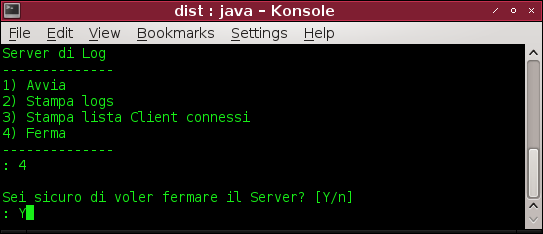
\includegraphics[width=1.0\textwidth]{images/server_di_log-10.png}
\vspace{-0.6cm}
\caption{Arresto Server di Log}
\end{figure}
\end{center}
\vspace{-1.0cm}
Con l'input Y il Server di Log viene terminato. L'applicativo Client \`e pensato per continuare a funzionare anche se il Server di Log viene fermato.

\subsection{Client}
Prima di avviare il Client assicurarsi che:
\begin{enumerate}
\item Il file configurazione.xml sia presente nella cartella da cui viene eseguito il Server di Log.
\item Il file configurazione.xsd sia presente nella cartella da cui viene eseguito il Server di Log.
\item Siano stati inseriti i parametri corretti nel file configurazioni.xml.
\end{enumerate}
Il Client pu\`o essere avviato da linea di comando con il seguente comando:
\lstset{language=bash}
\begin{lstlisting}[frame=single]
$ java -jar Client.jar
\end{lstlisting}
\textbf{Oppure \`e possibile utilizzare lo script .bat, vedi sezione 4.3.}\\
\\
Una volta avviato il Client, la prima finestra che viene mostrata all'utente \`e la seguente:
\begin{figure}[H]
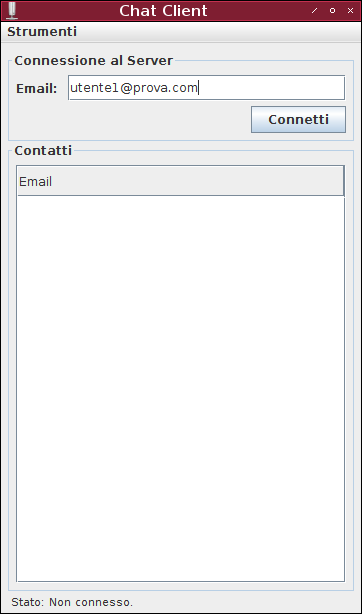
\includegraphics[height=1.2\textwidth]{images/client-1.png}
\vspace{-0.2cm}
\caption{Avvio Client}
\end{figure}
\clearpage
L'utente inserisce l'indirizzo email da utilizzare e si connette al servizio di messaggistica utilizzando il pulsante "Connetti":
\begin{figure}[H]
\vspace{-0.3cm}
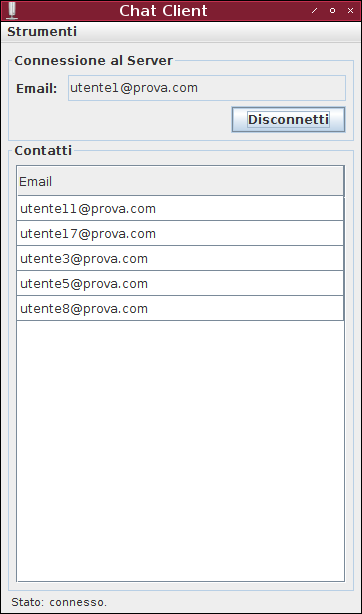
\includegraphics[height=1.2\textwidth]{images/client-2.png}
\vspace{-0.3cm}
\caption{Client connesso}
\end{figure}
\vspace{-0.3cm}
Non \`e possibile connettersi al servizio di messaggistica se il Server di Log non \`e stato avviato:
\begin{figure}[H]
\vspace{-0.3cm}
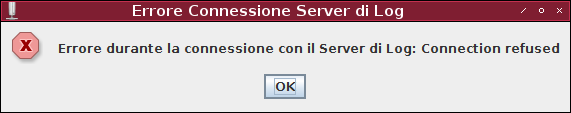
\includegraphics[width=1.0\textwidth]{images/client-18.png}
\end{figure}
\clearpage
Quando un nuovo Contatto si connette al servizio di messaggistica, viene aggiornata la lista dei Contatti connessi:
\begin{figure}[H]
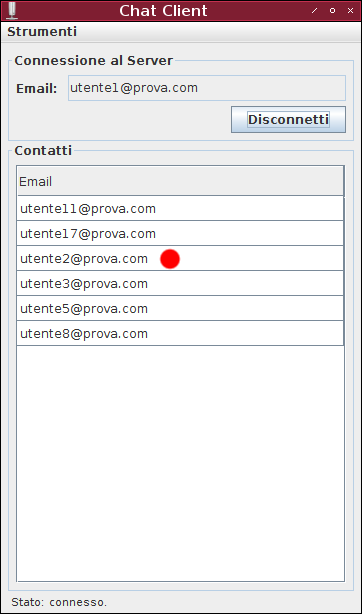
\includegraphics[height=1.2\textwidth]{images/client-3.png}
\vspace{-0.2cm}
\caption{Aggiornamento lista Contatti connessi}
\end{figure}
\clearpage
Con doppio click sul nome del Contatto \`e possibile aprire una nuova finestra di conversazione con esso:
\begin{figure}[H]
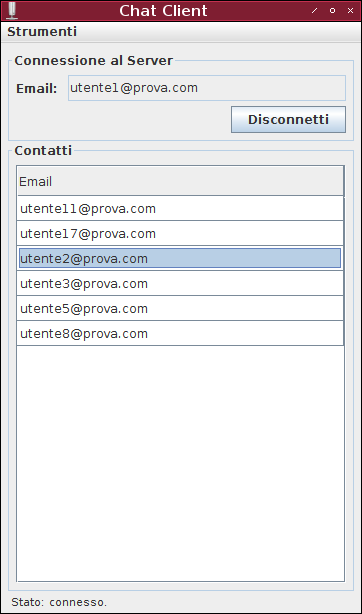
\includegraphics[height=0.9\textwidth]{images/client-4.png}
\\
\\
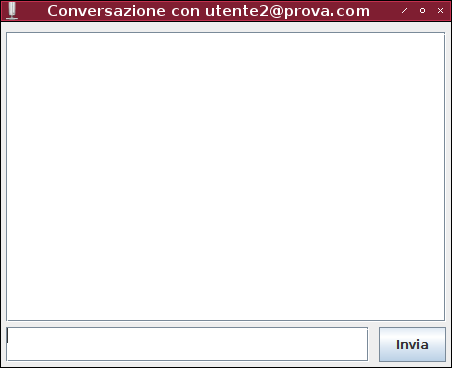
\includegraphics[width=0.6\textwidth]{images/client-5.png}
\vspace{-0.2cm}
\caption{Apertura Nuova conversazione}
\end{figure}
\clearpage
Ora i due utente possono iniziare lo scambio di messaggi utilizzando l'area di testo e il pulsante "Invia":
\begin{figure}[H]
\hspace{-2.0cm}
\begin{tabular}{cc}
  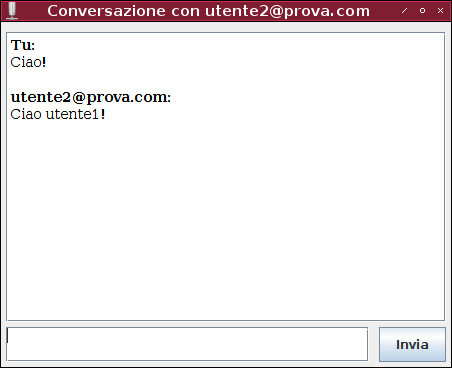
\includegraphics[width=80mm]{images/client-6.png} & 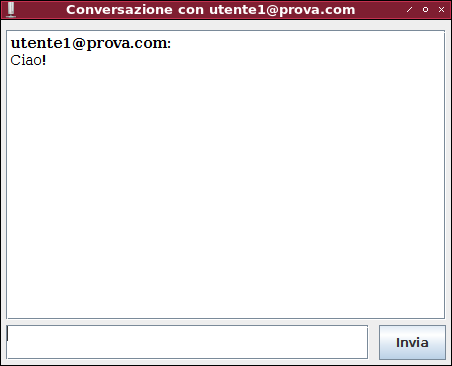
\includegraphics[width=80mm]{images/client-6-1.png} \\
  \\
  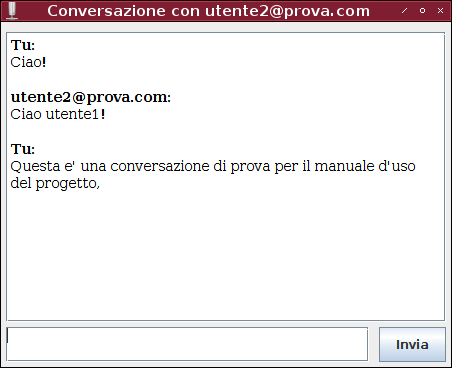
\includegraphics[width=80mm]{images/client-7.png}
\end{tabular}
\caption{Scambio di messaggi tra due Contatti}
\end{figure}
\clearpage
Quando viene chiusa una finestra di conversazione, vengono salvati in cache gli ultimi n messaggi scambiati, come indicato nel file di configurazione locale:
\begin{figure}[H]
\hspace{-2.0cm}
\begin{tabular}{cc}
  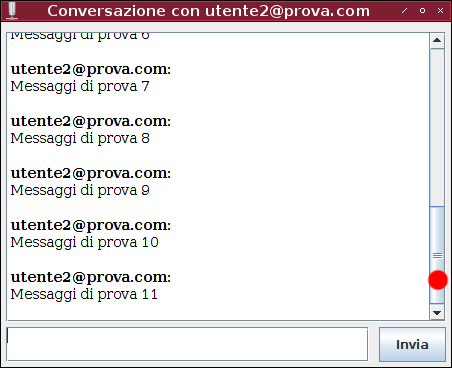
\includegraphics[width=80mm]{images/client-8.png} & 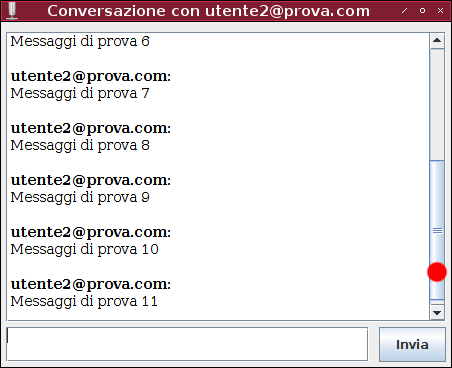
\includegraphics[width=80mm]{images/client-9.png}
\end{tabular}
\vspace{-0.5cm}
\caption{Caching messaggi scambiati}
\end{figure}
Quando il contatto con cui si conversa si disconnette, non \`e pi\`u possibile inviare messaggi nella finestra di conversazione:
\begin{figure}[H]
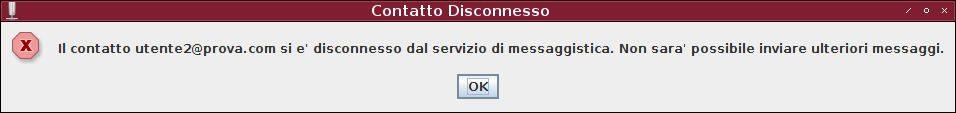
\includegraphics[width=1.2\textwidth]{images/client-10.png}
\\
\\
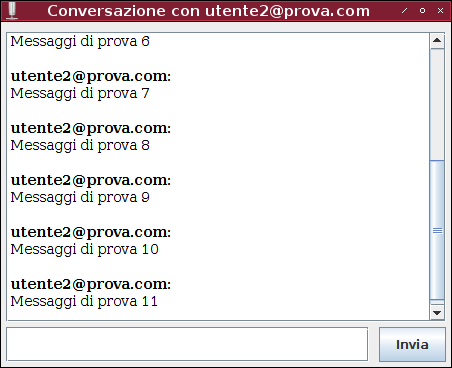
\includegraphics[width=0.6\textwidth]{images/client-11.png}
\vspace{-0.2cm}
\caption{Disconnessione Contatto}
\end{figure}
\clearpage
\hspace{-0.6cm}
Tramite il menu Strumenti $\rightarrow$ Statistiche, \`e possibile accedere alla finestra delle statistiche:
\begin{figure}[H]
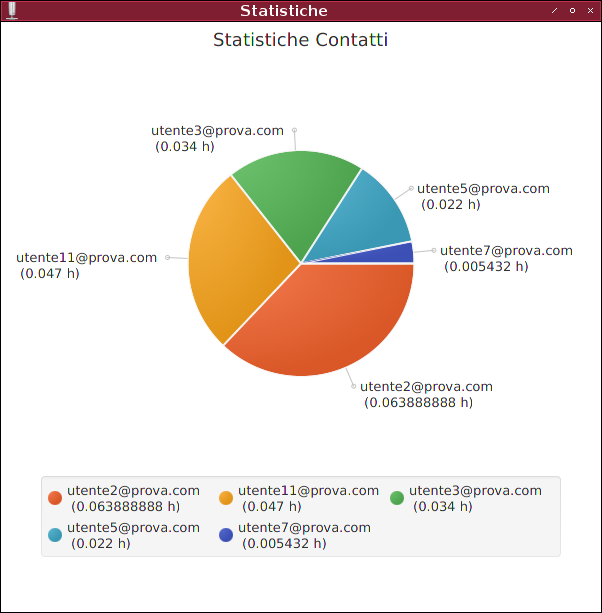
\includegraphics[width=1.0\textwidth]{images/client-12.png}
\vspace{-0.6cm}
\caption{Finestra Statistiche}
\end{figure}
Non \`e possibile accedere alla finestra delle statistiche se non si `e connessi al servizio di messaggistica:
\begin{figure}[H]
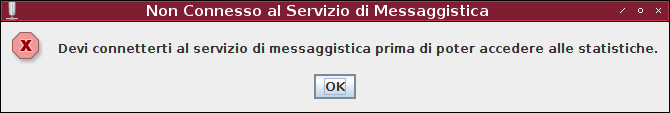
\includegraphics[width=1.0\textwidth]{images/client-17.png}
\vspace{-0.6cm}
\caption{Finestra Statistiche}
\end{figure}
\clearpage
Utilizzando il pulsante "Disconnetti" \`e possibile disconnettersi dal servizio di messaggistica.
\begin{figure}[H]
\hspace{-2.0cm}
\begin{tabular}{cc}
  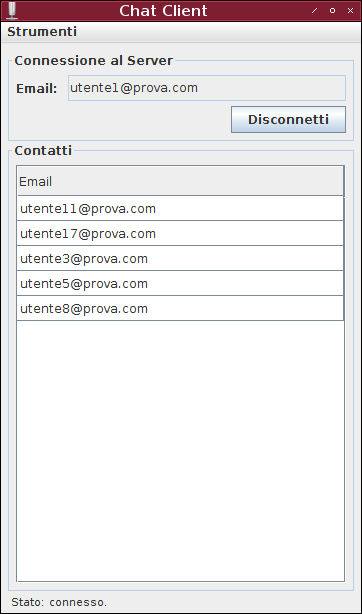
\includegraphics[width=80mm]{images/client-13.png} & 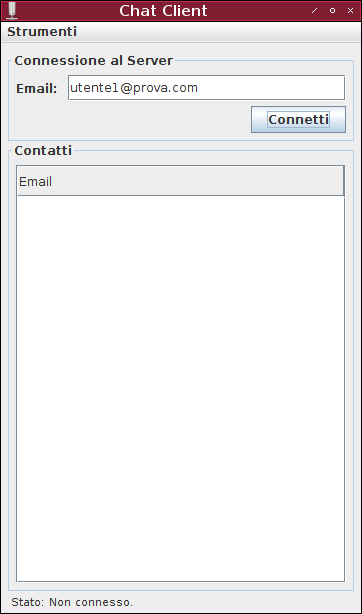
\includegraphics[width=80mm]{images/client-14.png}
\end{tabular}
\caption{Disconnessione dal servizio di messaggistica}
\end{figure}
Prima di chiudere la finestra principale del Client, viene chiesta conferma:
\begin{figure}[H]

\includegraphics[width=0.5\textwidth]{images/client-16.png}
\vspace{-0.2cm}
\caption{Finestra Statistiche}
\end{figure}

\subsection{Script bat}
Lo script bat "programmazione\_java.bat" pu\`o essere utilizzato su macchine con sistema operativo Windows per compilare i file sorgenti dei tre progetti e ottenere due file .jar che vengono poi eseguiti.\\
\\
Di seguito le screenshot relative all'utilizzo dello script .bat:\\
\begin{center}
\begin{figure}[H]
\vspace{-0.8cm}
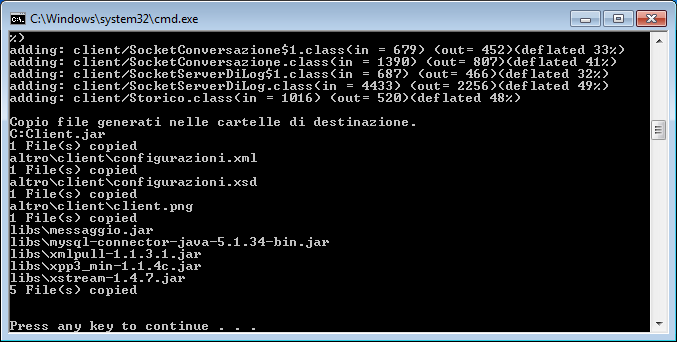
\includegraphics[width=1.0\textwidth]{images/script_bat-1.PNG}
\vspace{-0.7cm}
\caption{Esecuzione Script bat}
\end{figure}
\end{center}
\vspace{-1.4cm}
\begin{center}
\begin{figure}[H]
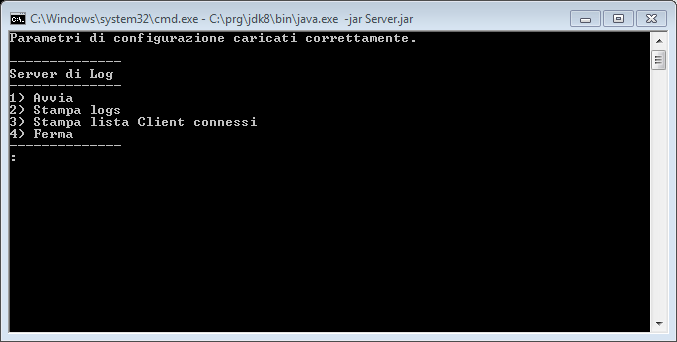
\includegraphics[width=1.0\textwidth]{images/script_bat-2.PNG}
\vspace{-0.7cm}
\caption{Script bat: Avvio Server di Log}
\end{figure}
\end{center}
\vspace{-1.4cm}
\begin{center}
\begin{figure}[H]
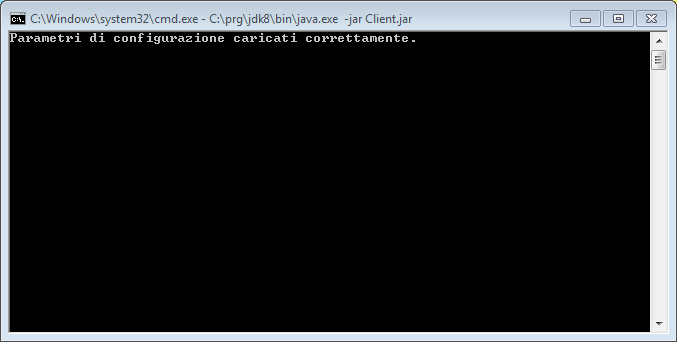
\includegraphics[width=1.0\textwidth]{images/script_bat-3.PNG}
\vspace{-0.7cm}
\caption{Script bat: Avvio Client}
\end{figure}
\end{center}
\begin{center}
\begin{figure}[H]
\vspace{-1.0cm}
\hspace{2.98cm}
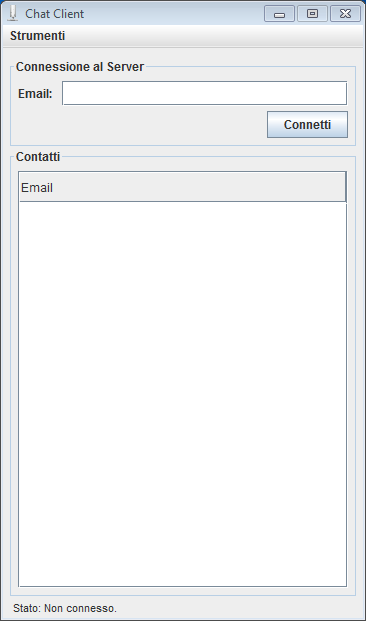
\includegraphics[width=0.5\textwidth]{images/script_bat-4.PNG}
\caption{Script bat: Avvio Client}
\end{figure}
\end{center}
%------------------------------------------------

%----------------------------------------------------------------------------------------
%	BIBLIOGRAPHY
%----------------------------------------------------------------------------------------

\newpage
\bibliographystyle{unsrt}

\bibliography{progetto_rambod_rahmani}

\nocite{*}

%----------------------------------------------------------------------------------------

\end{document}